\documentclass{Gharaei}
\usepackage{wrapfig}
\title{Vorlage UML, Betriebssysteme und Rechnernetze}
\author{Clarissa Röhrdanz, Jannes Schareitz \& Paul Kruse}
\date{26.05.2020}

\begin{document}
\maketitle
\newpage
\thispagestyle{empty}
\tableofcontents
\setcounter{page}{1}
\newpage
\section{1st Assignment}
A creature from outer space has conquered a space ship and has reached the earth. As it has 100 years of live remaining its goal is to replicate itself. Analyzing the climate on earth it concludes that it has to increase earth's average surface temperature by 5 degree. Researching the data base of the space ship it finds that the Global Warming Potential of $N_{2}O$ is highest and therefore discovers the easiest way to achieve its global warming goal to be the increase of dairy, beef, poultry and pork production on earth. This it supposes will lead to land degradation which is one of the main contributers for global warming. %20 words to go
\newpage
\section{2nd Assignment}
\subsection{Use case land degradation}
\begin{table}[H]
    \centering
    \caption{\textbf{Mains Success Scenario} for Land degradation}
    \begin{tabular}{l r l l}
        \textbf{Degradade Land} & & \\
         Main Success Scenario: & & \\
        & 1. & destroy forrest\\
         &2.& drain pleatlands\\

 &        3.& create soil\\
&         4.& use soil as pasture\\
  &      5.& use soil as croplands\\
   &     6.&intesive use of soil\\
    &   7.& ploughing up grasslands \\
     &  8.& changing pasture to croplands\\

      & 9.&  Loss of soil organic carbon\\
         \textbf{Extensions}\\

      &  & \begin{tabular}{r l l}
             
            9.a.& soil is lost:&  \\
            1. & carbon oxide is released \\
            2.& nitrous oxide is released \\
            3.& methane is released\\
         \end{tabular}
        
    \end{tabular}
\end{table}
The above table shows the Main Success Scenario (MSS) for Land degradation. The figure \ref{landDegradationGHG} below shows the use case diagram created from this scenario. The creature from out framework raises demand for dairy, poultry and other animal based nutrients thus affecting the food industry. The demand is directly handed to the farmer who produces these goods. As he can not satisfy the rising demand with his current ressources a demand arises for more soil. Handed to the Drainer and the Forester these actors in turn take actions which lead to more soil. These actions are represented by use cases in the Land Degradation system. The farme too takes actions he uses its ressources, namely the soil, for two food generating activities: as pasture and as croplands. This use of soil leads to its loss which in tun leads to GHG releases.
\begin{figure}[H]
    \centering
    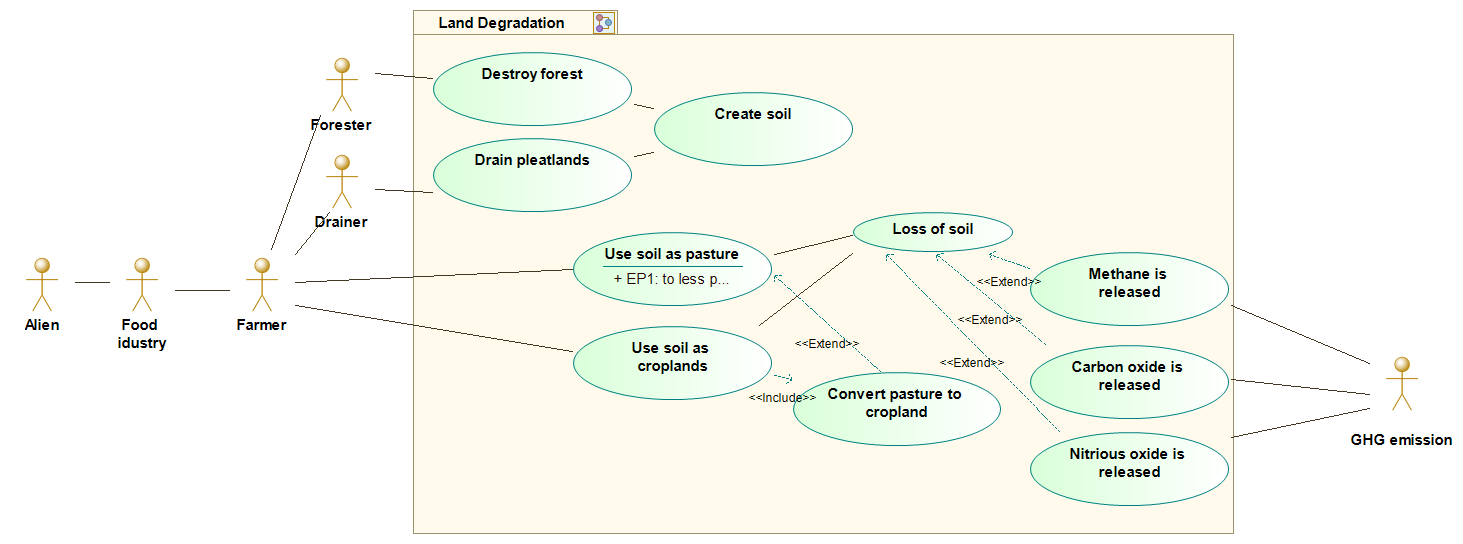
\includegraphics[width=\textwidth-2cm]{2ndUCdiagramm.png}
    \caption{Role of land degradation in GHG emission}
    \label{landDegradationGHG}
\end{figure}
 
\section{3rd Assignment}
\subsection{3A}
\subsection{3B}
\subsection{3T}
\begin{figure}[H]
    \centering
    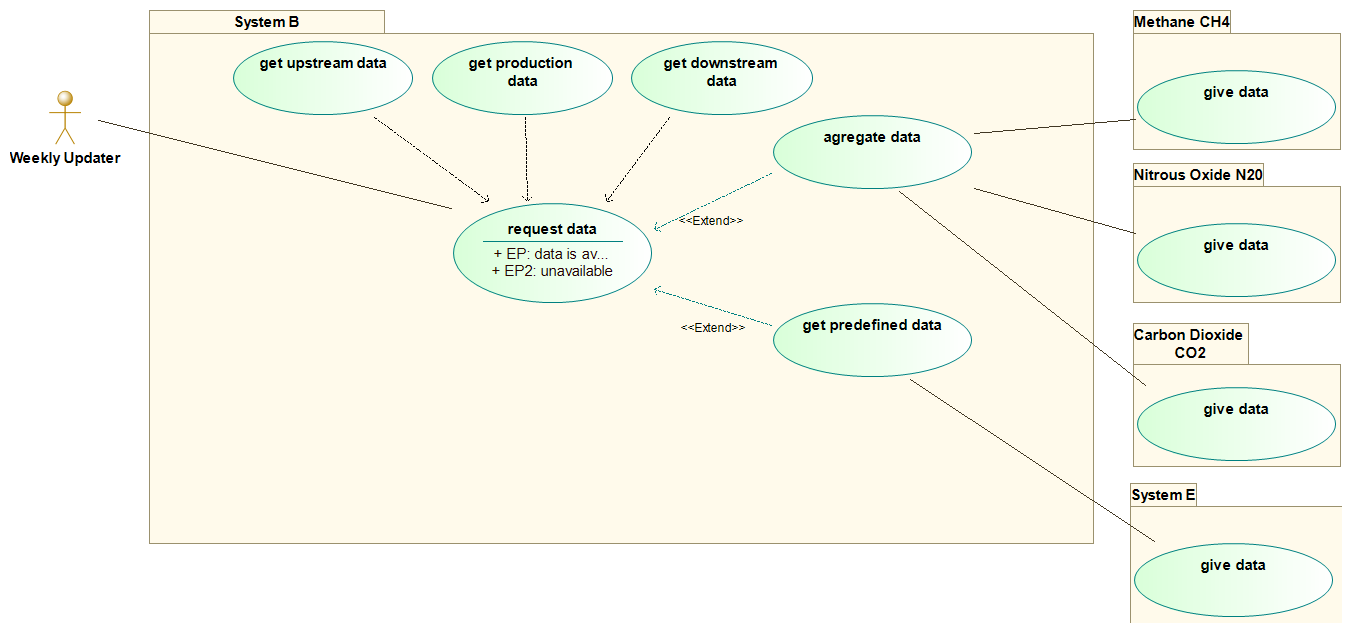
\includegraphics[height=\textheight-4cm]{3rdBUCdiagramm.png}
    \caption{System B aggregating data}
    \label{SysB}
\end{figure}
\section{4th Assignment}
\subsection{4A}
\subsection{4B}
\begin{tabular}{p{15cm} l} 
 \begin{tabular}{p{15cm}}
    There are two expansion regions in this activity diagram. The first was chosen as parallel because for every kind of green house gas the requests can be executed at the same time. These data is collected from different systems. 
    In each such system there is data from different ressources. These are collected iteratively or each GHG production stream. Thus I chose the iterative type of expansion.
 \end{tabular} &  
 \begin{tabular} {l}
    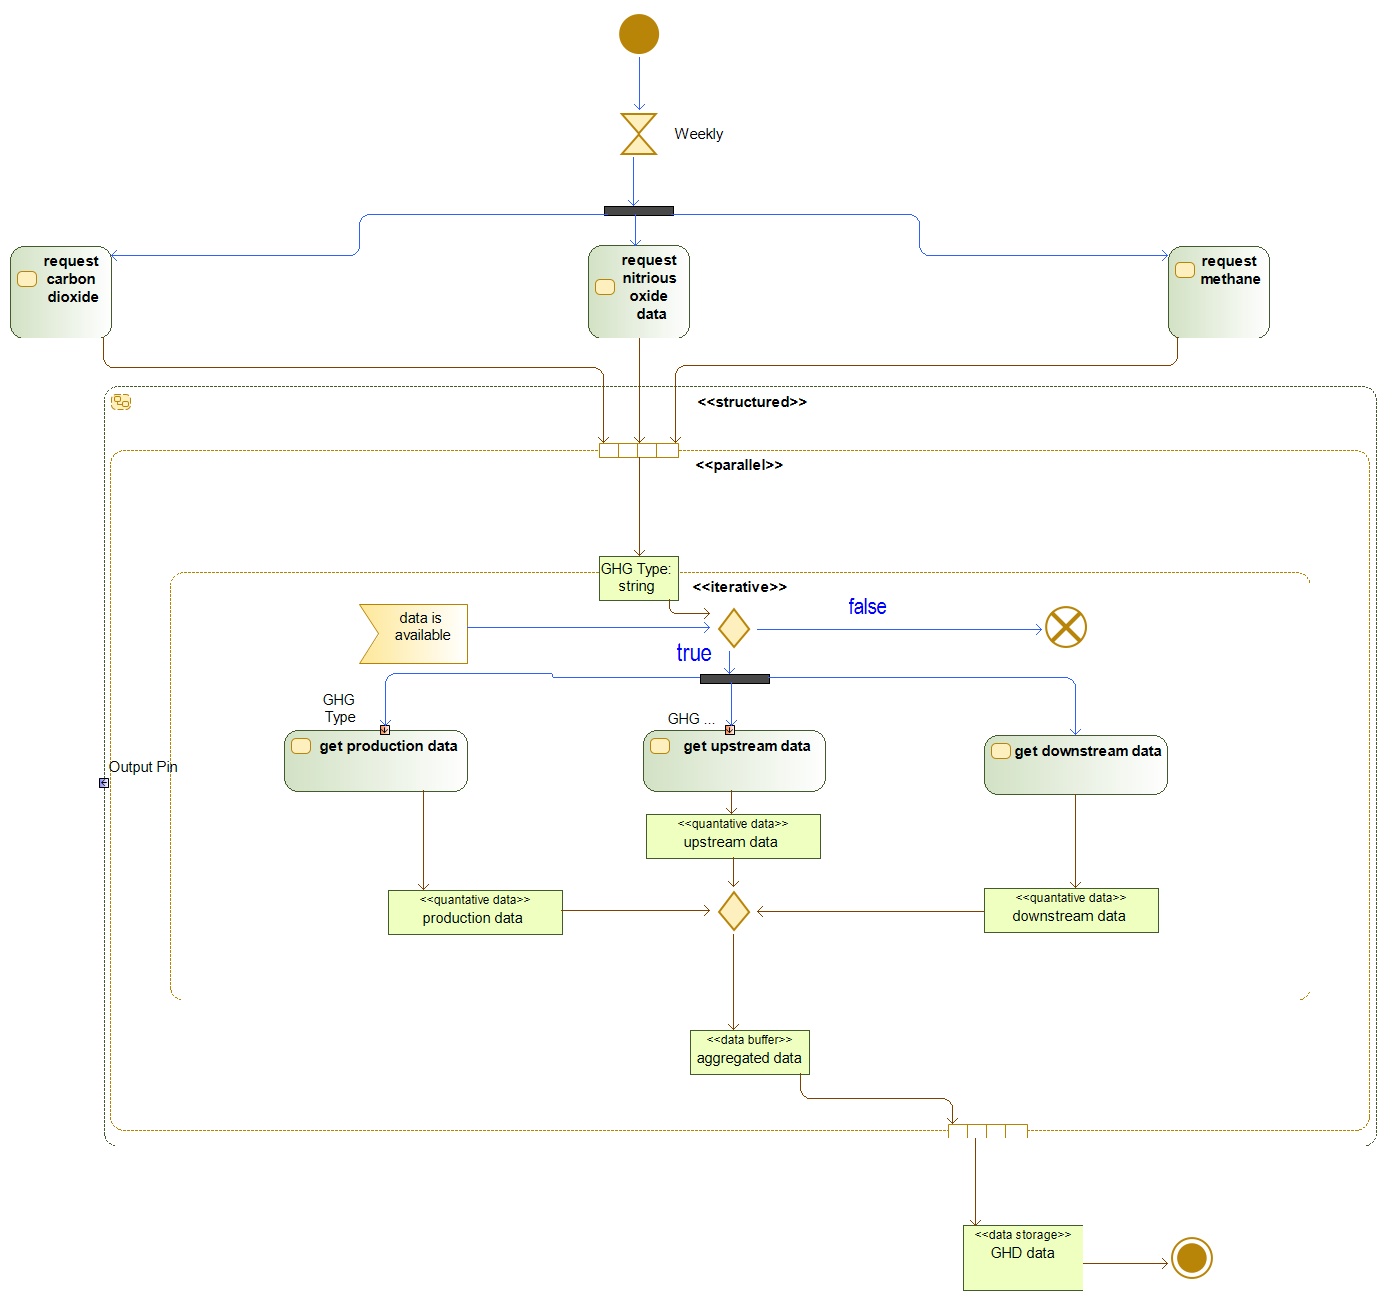
\includegraphics[height=0.60\textheight]{4vactivitydiagramm.png}
    \\ 
    Figure x: {Activity diagram for UC aggregate data (3B)}
 \end{tabular}
\end{tabular}
\subsection{4T}
\section {Erklärung}
Hiermit versichern wir, dass wir nicht Teile einer fremden Arbeit, insbesondere solche aus dem Internet bzw. von hier nicht angegebenen Kommilitonen oder ehemaligen Teilnehmern an der betroffenen Lehrveranstaltung, zur Bewertung einreichen. Ebenso versichern wir, dass die Arbeit nicht, auch nicht auszugsweise, bereits für eine andere Prüfung angefertigt wurde. Wir  haben  verstanden,  dass  es  zulässig  ist,  dass  wir  die  Arbeit  unter  Heranziehung  relevanter  Quellen  erstellen.  Wikipedia  ist  jedoch  keine  relevante  Quelle. Alle wörtlich oder sinngemäß den Arbeiten anderer entnommenen Stellen haben wir unter Angabe der Quellen kenntlich gemacht. Dies gilt ebenso für Zeichnungen, bildliche Darstellungen, Skizzen, Tabellen und dergleichen.  Uns ist bewusst, dass wahrheitswidrige Angaben als Täuschungsversuch behandelt werden und dass bei einem Täuschungsverdacht sämtliche Verfahren der Plagiatserkennung angewandt werden können.
\end{document}